\subsection{Individual primary outcomes}

\begin{center}

\begin{tabular}{rrrrrr}

\toprule

Seed & $T_{\rm fit}^{64}$ & $T_{\rm gen}^{64}$ & $T_{\rm fit}^{256}$ & $T_{\rm gen}^{256}$ & $\tau^{256}-\tau^{64}$ \\

\midrule

10 & 300 & $>29{,}800$ & 100 & 11,300 & -18,500 \\

11 & 300 & $>29{,}800$ & 100 & 11,100 & -18,700 \\

12 & 300 & $>29{,}800$ & 100 & 10,300 & -19,500 \\

13 & 300 & $>29{,}800$ & 100 & 11,700 & -18,100 \\

14 & 300 & $>29{,}800$ & 100 & 13,500 & -16,300 \\

\bottomrule

\end{tabular}

\end{center}

\subsection{Threshold sensitivity}

All entries give sustained held-out event times in seed order 10--14; a dash means not confirmed by $H=29{,}800$.

At threshold 90\% and width 64: --, --, --, --, --.

At threshold 90\% and width 256: 9,000, 8,800, 8,300, 9,300, 9,500.

At threshold 95\% and width 64: --, --, --, --, --.

At threshold 95\% and width 256: 11,300, 11,100, 10,300, 11,700, 13,500.

At threshold 99\% and width 64: --, --, --, --, --.

At threshold 99\% and width 256: 26,700, 15,000, 13,300, 16,200, 20,700.

\subsection{Matched arithmetic budget proxy}

Width 64, checkpoint 30,000: mean held-out accuracy 0.716 [0.685, 0.750] (95\% seed bootstrap interval); individual values 0.715, 0.694, 0.775, 0.730, 0.665.

Width 128, checkpoint 15,000: mean held-out accuracy 0.928 [0.910, 0.950] (95\% seed bootstrap interval); individual values 0.933, 0.967, 0.925, 0.900, 0.917.

Width 256, checkpoint 7,500: mean held-out accuracy 0.830 [0.796, 0.862] (95\% seed bootstrap interval); individual values 0.867, 0.807, 0.871, 0.769, 0.834.

\begin{figure}[h]

\centering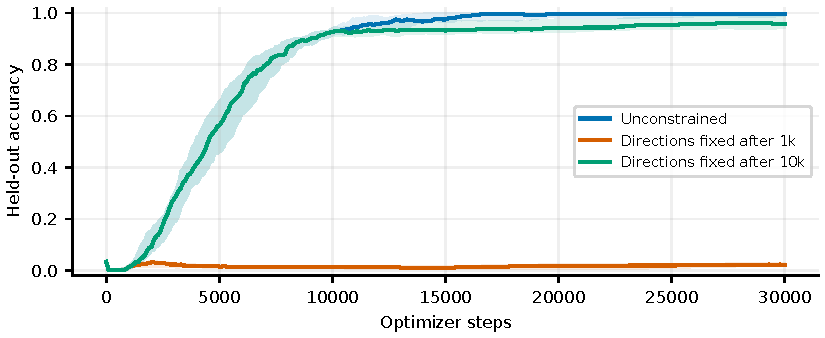
\includegraphics[width=\linewidth]{figures/feature_freezing.pdf}

\caption{Exploratory feature-direction freezing at width 256. Curves are medians with full seed ranges. The first 1,000 or 10,000 steps exactly match the unconstrained reference; subsequent optimization retains the fixed ReLU feature directions, while magnitudes and readout weights remain trainable.}

\label{fig:freezing}

\end{figure}

\subsection{Event proportions and computational cost}

Exact Clopper--Pearson intervals for every cell are in \texttt{generated/summary.json}; these intervals describe seed-level event probabilities under the complete seed-and-split procedure. Five seeds give limited resolution and no rare-event guarantee.

The 255 distinct formal runs consume 2.54 measured process CPU hours in training/evaluation. Interpreter startup, pilots, the interrupted launcher, analysis, and compilation are excluded from that total; individual measured wall times are in the raw JSON and per-run CSV.
